%%%%%%%%%%%%%%%%%%%%%%%%%%%%%%%%%%%%%%%%%%%%%%%%%%%%%%%%%%%%%%%%%%%%%%
% UMB-CS114-2015F: Introduction to Programming in Java
% Copyright 2015 Pejman Ghorbanzade <pejman@ghorbanzade.com>
% Creative Commons Attribution-ShareAlike 4.0 International License
% More info: https://github.com/ghorbanzade/UMB-CS114-2015F
%%%%%%%%%%%%%%%%%%%%%%%%%%%%%%%%%%%%%%%%%%%%%%%%%%%%%%%%%%%%%%%%%%%%%%

\def \topDirectory {../..}
\def \texDirectory {\topDirectory/src/main/tex}

\documentclass[10pt, compress]{beamer}

\usepackage{\texDirectory/template/style/directives}
% -----------------------------------------------------------------------------
% The MIT License (MIT)
%
% Copyright (c) 2015 Pejman Ghorbanzade
%
% Permission is hereby granted, free of charge, to any person obtaining a copy
% of this software and associated documentation files (the "Software"), to deal
% in the Software without restriction, including without limitation the rights
% to use, copy, modify, merge, publish, distribute, sublicense, and/or sell
% copies of the Software, and to permit persons to whom the Software is
% furnished to do so, subject to the following conditions:
%
% The above copyright notice and this permission notice shall be included in
% all copies or substantial portions of the Software.
%
% THE SOFTWARE IS PROVIDED "AS IS", WITHOUT WARRANTY OF ANY KIND, EXPRESS OR
% IMPLIED, INCLUDING BUT NOT LIMITED TO THE WARRANTIES OF MERCHANTABILITY,
% FITNESS FOR A PARTICULAR PURPOSE AND NONINFRINGEMENT. IN NO EVENT SHALL THE
% AUTHORS OR COPYRIGHT HOLDERS BE LIABLE FOR ANY CLAIM, DAMAGES OR OTHER
% LIABILITY, WHETHER IN AN ACTION OF CONTRACT, TORT OR OTHERWISE, ARISING FROM,
% OUT OF OR IN CONNECTION WITH THE SOFTWARE OR THE USE OR OTHER DEALINGS IN
% THE SOFTWARE.
% -----------------------------------------------------------------------------

\course{id}{CS114}
\course{name}{Introduction to Java}
\course{venue}{Mon/Wed, 5:30 PM - 6:45 PM}
\course{semester}{Fall 2015}
\course{department}{Department of Computer Science}
\course{university}{University of Massachusetts Boston}

\instructor{name}{Pejman Ghorbanzade}
\instructor{title}{}
\instructor{position}{Student Instructor}
\instructor{email}{pejman@cs.umb.edu}
\instructor{phone}{617-287-6419}
\instructor{office}{S-3-124B}
\instructor{office-hours}{Mon/Wed 16:00-17:30}
\instructor{address}{University of Massachusetts Boston, 100 Morrissey Blvd., Boston, MA}

\usepackage{\texDirectory/template/style/beamerthemeUmassLecture}
\doc{number}{3}
%\setbeamertemplate{footline}[text line]{}

\begin{document}
\prepareCover

\section{Course Administration}

\begin{slide}
	\begin{itemize}
		\item[] 19/40 user accounts at \href{http://www.ghorbanzade.com}{Course Website} created so far.
	\end{itemize}
\end{slide}

\begin{slide}
	\begin{block}{Overview}
		\begin{itemize}
			\item[] Java Programming Architecture
			\item[] Java Hello World Program
			\item[] Command-line Arguments
		\end{itemize}
	\end{block}
\end{slide}

\section{Java Architecture}

\begin{slide}
	\begin{block}{Goals}
		\begin{columns}
			\begin{column}{0.7\textwidth}
			\begin{itemize}
				\item[] To be simple, object-oriented and familiar
				\item[] To be robust and secure
				\item[] To be architecture-neutral and portable
				\item[] To execute with high performance
				\item[] To be interpreted, threaded and dynamic
			\end{itemize}
			\end{column}
			\begin{column}{0.3\textwidth}
			\begin{figure}
				
\includegraphics[width=\textwidth]{\texDirectory/template/images/logo.png}
			\end{figure}
			\end{column}
		\end{columns}
	\end{block}
\end{slide}

\begin{slide}
	\begin{block}{Applications}
		\begin{itemize}
			\item[] Java Applets
			\item[] Java Servlets
			\item[] Java Server Pages
			\item[] Java Database Connectivity
		\end{itemize}
	\end{block}
\end{slide}

\begin{slide}
	\begin{block}{Execution Procedure}
		\begin{itemize}
			\item[] Java code is compiled to Java Bytecode
			\item[] Java bytecode is interpreted by Java Virtual Machine
			\item[] Java Virtual Machine converts Java Bytecode to machine code.
			\item[] Sacrifice speed to achieve portability
		\end{itemize}
	\end{block}
\end{slide}

\section{Java Hello-World Program}

\begin{slide}
	\begin{figure}
		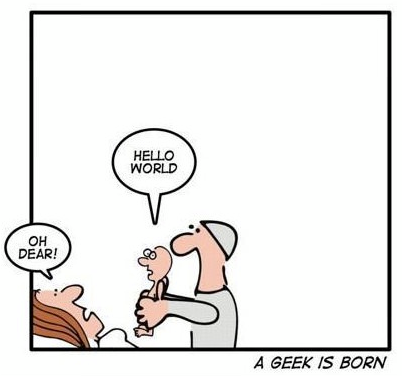
\includegraphics[height=0.7\textheight]{\texDirectory/template/images/helloworld.png}
	\end{figure}
\end{slide}

\begin{slide}
	\begin{block}{HelloWorld.java}
		\begin{minted}[fontsize=\small, linenos, firstnumber=1]{java}
			public class HelloWorld {
			    public static void main(String[] args) {
			        System.out.println("Hello World!");
			    }
			}
		\end{minted}
	\end{block}
	\pause
	\begin{block}{Key Words}
		\begin{columns}
		\begin{column}{0.5\textwidth}
			\begin{itemize}
				\item[] Classes
				\item[] Methods
			\end{itemize}
		\end{column}
		\begin{column}{0.5\textwidth}
			\begin{itemize}
				\item[] Statements
				\item[] Arguments
			\end{itemize}
		\end{column}
		\end{columns}
	\end{block}
\end{slide}

\begin{slide}
	\begin{block}{Terminal}
		\begin{minted}[fontsize=\small,tabsize=8]{bash}
			$ javac HelloWorld.java
			$ java HelloWorld
			Hello World!
		\end{minted}
	\end{block}
\end{slide}

\section{Command-line Arguments}

\begin{slide}
	\begin{block}{SayHello.java}
		\begin{minted}[fontsize=\small,tabsize=8]{java}
			public class SayHello {
			    public static void main(String[] args) {
			        System.out.println("Hello! How are you?");
			    }
			}
		\end{minted}
	\end{block}
	\begin{block}{Terminal}
		\begin{minted}[fontsize=\small,tabsize=8]{bash}
			$ javac SayHello.java
			$ java SayHello
			    Hello! How are you?
		\end{minted}
	\end{block}
\end{slide}

\begin{slide}
	\begin{block}{SayHello.java}
		\begin{minted}[fontsize=\small,tabsize=8]{java}
			public class SayHello {
			    public static void main(String[] args) {
			        System.out.println("Hello " + args[0] + "! ");
			        System.out.println("How are you?");
			    }
			}
		\end{minted}
	\end{block}
	\begin{block}{Terminal}
		\begin{minted}[fontsize=\small,tabsize=8]{bash}
			$ java SayHello Pejman
			Hello Pejman! How are you?
			$ java SayHello 12@#1
			Hello 12@#1! How are you?
		\end{minted}
	\end{block}
\end{slide}

\begin{slide}
	\begin{block}{Motivation}
		\begin{itemize}
			\item[] Efficient Interthread Communication in JVM by means of piping and redirection
		\end{itemize}
	\end{block}
	\begin{block}{Advantages}
		\begin{itemize}
			\item[] Provides a way to give input to program
			\item[] Simple to begin with
		\end{itemize}
	\end{block}
	\begin{block}{Disadvantages}
		\begin{itemize}
			\item[] All user-specified arguments to be given before execution of program
			\item[] All arguments are of type String
		\end{itemize}
	\end{block}
\end{slide}

\plain{}{Keep Calm\\and\\Start Writing Code}

\end{document}
